%%%%%%%%%%%%%%%%%%%%%%%%%%%%%%%%%%%%%%%%%
% Short Sectioned Assignment
% LaTeX Template
% Version 1.0 (5/5/12)
%`
% This template has been downloaded from:
% http://www.LaTeXTemplates.com
%
% Original author:
% Frits Wenneker (http://www.howtotex.com)
%
% License:
% CC BY-NC-SA 3.0 (http://creativecommons.org/licenses/by-nc-sa/3.0/)
%
%%%%%%%%%%%%%%%%%%%%%%%%%%%%%%%%%%%%%%%%%

%----------------------------------------------------------------------------------------
%	PACKAGES AND OTHER DOCUMENT CONFIGURATIONS
%----------------------------------------------------------------------------------------

\documentclass{article}

\usepackage[T1]{fontenc} % Use 8-bit encoding that has 256 glyphs
%\usepackage{fourier} % Use the Adobe Utopia font for the document - comment this line to return to the LaTeX default
\usepackage[english]{babel} % English language/hyphenation
\usepackage{amsmath,amsfonts,amsthm, amssymb} % Math packages
\usepackage{sectsty} % Allows customizing section commands
\usepackage{tikz-cd} % Allows for commutative diagrams
\usepackage[]{enumerate} %Changing enumerate environment
\usepackage{mathrsfs} %fonts?
\usepackage{cancel} % for pretty slashes
\usepackage{graphicx}

\graphicspath{{figures/}}

\begin{document}
	
	\title{Combinatorics and Computation Notes}
	\author{Nate Schieber}
	\date{11/15/2019}
	\maketitle
	
	\section{Statistical Mechanics on the Hexagonal Graph}
	
	\hspace{1cm} Last time we saw a specific example of statistical mechanics that used the Dimer Model and a single parameter corresponding to the temperature of a particular state of a particular system. Specifically, the temperature was determined by a weight function $w: E \rightarrow \mathbb{R}$ where $E$ is the edge set of the graph. Though the same construction works for any bipartite graph, we will continue to work with the bipartite hexagon graph $G(a,b,c)$. Figure \ref{fig:hexagraph} shows $G(3,2,3)$. 
	
	

	\begin{figure}[h]
\begin{minipage}{\textwidth}
	\begin{center}
 	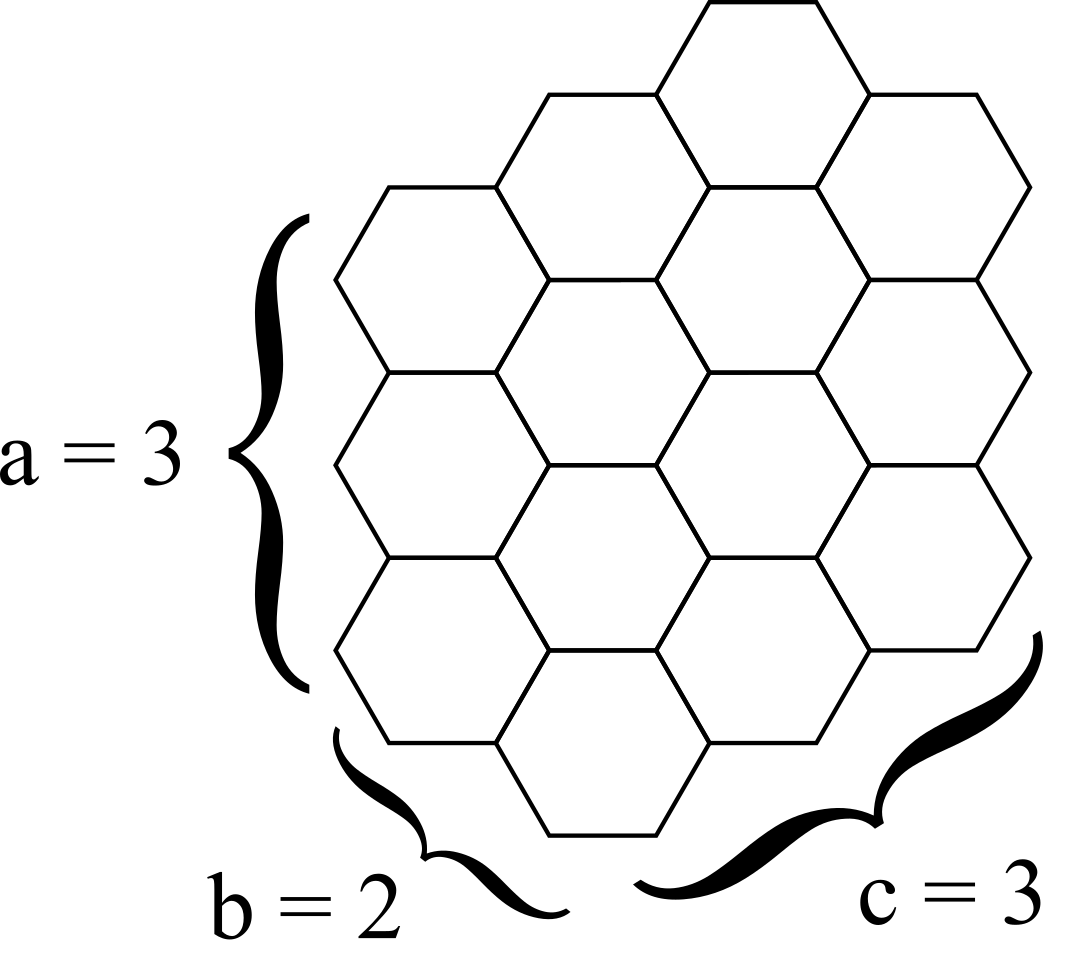
\includegraphics[width=6cm]{hexagraph.png}
  	\caption{The Hexagonal Graph $G(3,2,3)$}
	 \label{fig:hexagraph}
 	 \end{center}
 \end{minipage}	
\end{figure} 

	
	Though we will not prove it, we have the following theorem due to MacMahon in the early twentieth century. 
	%\begin{minipage}{.9\textwidth}
	\subsection{Theorem:} There are
	$$
	\prod_{
	1 \leq i \leq a, 1 \leq j \leq b, 1 \leq k \leq c} \frac{i+j+k-1}{i+j+k-2} 
	$$
	perfect matchings on $G(a,b,c)$. 
	%\end{minipage}
	
	
\subsection*{Dimer Model and Plane Partitions}

\hspace{1cm} Recall that we were able to translate the dimer model on a hexagonal grid to one of plane partitions composed of rhombuses as shown in Figure \ref{fig:honey_rhombus}. 	
	\begin{figure}[h]
\begin{minipage}{\textwidth}
	\begin{center}
 	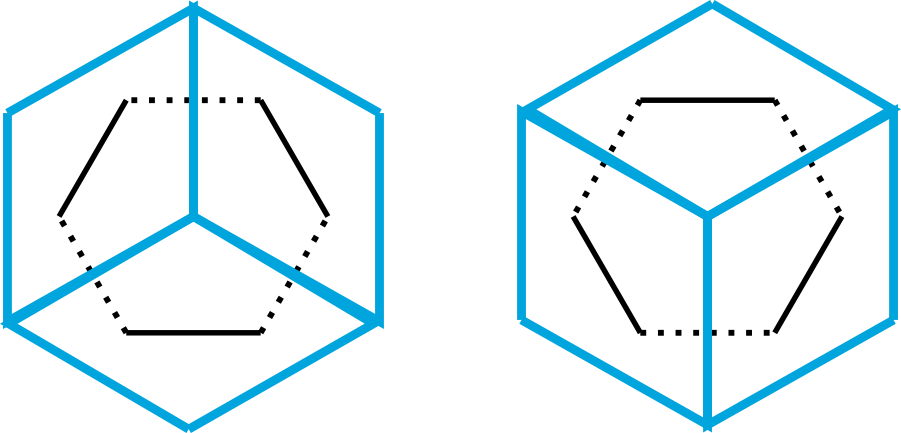
\includegraphics[width=6cm]{honey_rhombus.png}
  	\caption{}
	 \label{fig:honey_rhombus}
 	 \end{center}
 \end{minipage}	
\end{figure} 
We will now examine the specific case that our hexagonal grid is $G(a,b,c)$. 

\subsection{Definition:} A \textit{plane partition} is an array 
$$
(a_{ij})_{1 \leq i \leq a, \hspace{.5mm} 1 \leq j \leq b, \hspace{.5mm}  0 \leq a_{ij} \leq c}
$$ 
of natural numbers that is non-increasing in both indices. More explicitly,
$$
a_{ij} \geq a_{i(j+1)} \hspace{1cm} a_{ij} \geq a_{(i+1)j}.
$$
We can interpret these as describing how a certain number of boxes are stacked in the corner of a room. We only consider configurations in which there are no hidden boxes and this accounts for the non-increasing condition. The parameters $a,b,$ and $c$ in this context describe the dimensions of the room in which the boxes are to be stacked. Figure \ref{fig:box_stack} shows the $3 \times 2 \times 3$ plane partition 
$$
\begin{pmatrix}
3 & 3\\
3 & 3 \\
2 & 2
\end{pmatrix}
$$
realized as a stack of boxes. 
	\begin{figure}[h]
\begin{minipage}{\textwidth}
	\begin{center}
 	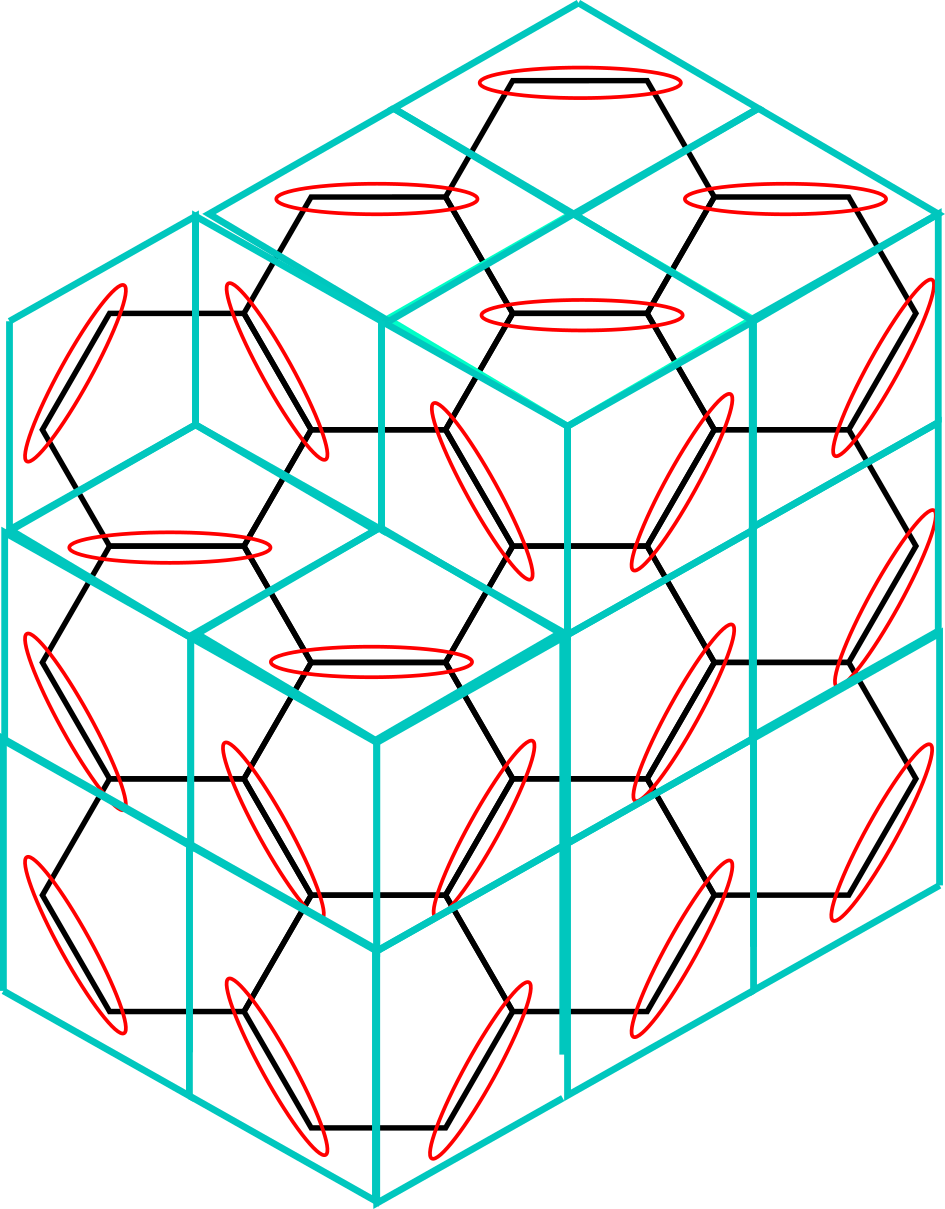
\includegraphics[width=6cm]{box_stack_1.png}
  	\caption{$3 \times 2 \times 3$ Boxed Plane Partition}
	 \label{fig:box_stack}
 	 \end{center}
 \end{minipage}	
\end{figure} 
A plane partition defined on $G(a,b,c)$ is called a \textit{$a\times b \times c$ boxed plane partition}. 

Recall now that last time we defined a weight function on the perfect matchings on $G(a,b,c)$ where diagonal edges were given weight $1$ and horizontal edges were given weight $q^t$ where $t$ is the number of horizontal edges below the one in question. Translating this into box-stacking gives us a generating function for the number of perfect matchings on $G(a,b,c)$. Let $P$ be the set of all $a \times b \times c$ boxed plane partitions and for $\pi \in P$ let $b(\pi)$ represent the number of boxes in $\pi$. Then
$$
Z(q) = K \sum_{\pi \in P} q^{b(\pi)} = K\sum e^{b(\pi) * \log(q)}.
$$
This formula can then be manipulated to show that
$$
Z(q) = K \prod_{1 \leq i \leq a,  1 \leq j \leq b,  1 \leq k \leq c} \frac{(1-q)^{i+j+k-1}}{1-q^{i+j+k-2}},
$$
a result again due to MacMahon. 


\section{Statistical Mechanics and Box Stacking}

\hspace{1cm} In statistical mechanics, the configuration of a system with minimal energy is called the \textit{ground state} of that system. As in our box stacking example the energy equals the number of boxes stacked, the ground state is an empty room. 

More generally, we are interested in how and when a system changes state. That is, where and under what conditions does the system experience a phase change. To explore this, we will need to recall that if $K$ is the Kasteleyn matrix for $G(a,b,c)$ then
$$
(K^{-1})_{i,j} = \mathbb{P}\{\text{edge $\overline{ij}$ is in a random perfect matching} \}.
$$
The entries of $K^{-1}$ are thus the \textit{edge placement probabilities} of the graph. In statistical mechanics, these entries are called \textit{$1$-point correlation functions}. This definition generalizes to $n$-point correlation functions, which are defined by choosing $n$ edges in a graph $e_1, \dots, e_n$ and then computing
$$
\mathbb{P} \{e_1, \dots, e_n \text{ are all in a given random perfect matching}\}. 
$$

These correlation functions serve as a main tool in examining phase transitions, particularly in large graphs. For example, as $a,b,$ and $c$ become large, a generic matching on $G(a,b,c)$ takes the form shown in Figure \ref{fig:gen_hex} where inside the red circle the matching appears random and outside the circle it appears deterministic. In particular, outside the circle the matching represents the ground state, which we can interpret either as a lack of boxes outside the circle, or as only the horizontal edges of each hexagon being selected by the matching. 
	\begin{figure}[h]
\begin{minipage}{\textwidth}
	\begin{center}
 	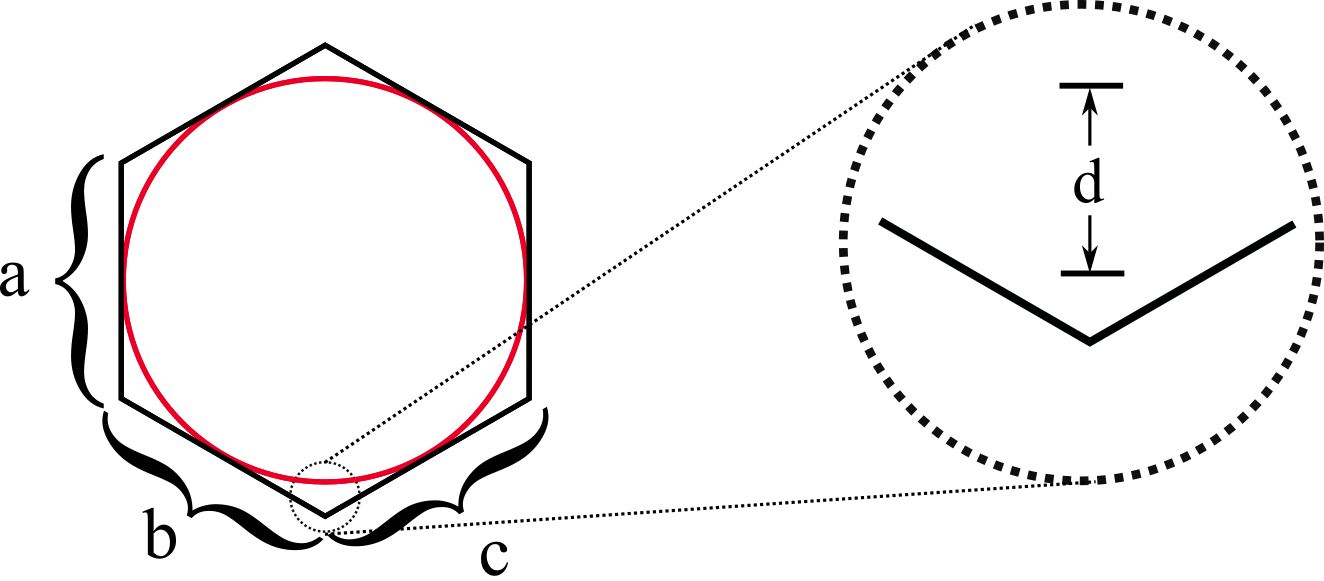
\includegraphics[width=\textwidth]{generic_hex.png}
  	\caption{Generic Perfect Matching on $G(a,b,c)$}
	 \label{fig:gen_hex}
 	 \end{center}
 \end{minipage}	
\end{figure} 	
	
	The boundary defined by the dotted circle represents the phase transition in which we are interested, the system taking on a regular, low-energy pattern on one side, and a random assortment on the other. We can now use the $1$-point correlation functions to study this transition. 
	
	To do so, we choose two horizontal edges near the boundary of the graph as shown in the diagram. Let $e_1$ represent the edge nearer the boundary and $e_2$ the edge further. Keeping $e_1$ fixed, we can vary $e_2$ allowing the distance $d$ between them to increase. We can then study the one point correlation function between $e_1$ and $e_2$ as a function of $d$, which we denote as $f(d)$. 
	
	For small $d$, we expect $f(d)$ to fall near $1$ as both edges are in the ground state matching. That is, these edges should stay correlated within the deterministic region outside of the red circle. On the other hand, as $d$ increases so that $e_2$ now falls within the random region, we should expect $f(d)$ to approach
	$$
	\mathbb{P}\{e_1\text{ is in the perfect matching}\} * \mathbb{P}\{e_2\text{ is in the perfect matching}\}
	$$
	indicating the independence of the edges. We should also expect polynomial decay of the values $f(d)$ takes as $a,b,$ and $c$ increase without bound. 
	
	 
	
	
	
	
	
	
\end{document}
	
	
	
	
	
	
	
\end{document}	
	
	
